	\section*{Exercice 3 (5 points)}
	
	\subsection*{Partie A}
	
	\subsubsection*{1. Calculer $P(B \cap S)$}
	
	On peut dresser un arbre pondéré de probabilités :
	
	\begin{tikzpicture}
	[level 1/.style={level distance=2cm,
		sibling distance=3cm},
	level 2/.style={level distance=2.5cm,
		sibling distance=1.5cm}]
	\node {} [grow'=right]
	child {node {$S$}
		child {node {$B$}
			edge from parent node[above] {$\dfrac34$}
		}
		child {node {$\overline B$}
			edge from parent node[below] {$\dfrac14$}
		}
		edge from parent node[above] {$\dfrac12$}
	}
	child {node {$\overline S$}
		child {node {$B$}
			edge from parent node[above] {$\dfrac18$}
		}
		child {node {$\overline B$}
			edge from parent node[below] {$\dfrac78$}
		}
		edge from parent node[below] {$\dfrac12$}
	}
	;
\end{tikzpicture}

	
	On a $P(B \cap S) = P(S \cap B) = P(S) \times P_S(B) = \dfrac{1}{2} \times \dfrac{3}{4} = \dfrac{3}{8}$.
	
	\subsubsection*{2. Déterminer la probabilité que le groupe de copains réponde correctement à la question posée}
	
	D’après la loi des probabilités totales on a :
	\[
	P(B) = P(B \cap S) + P(B \cap \overline{S}) = \dfrac{1}{2} + \dfrac{1}{2} \times \dfrac{1}{8} = \dfrac{3}{8} + \dfrac{1}{16} = \dfrac{6}{16} + \dfrac{1}{16} = \dfrac{7}{16}
	\]
	
	\subsubsection*{3. Les évènements $S$ et $B$ sont-ils indépendants ?}
	
	On a avec $P(S) = \dfrac{1}{2}$ :
	\[
	P(B \cap S) = \dfrac{3}{8} \text{ et } P(B) \times P(S) = \dfrac{7}{16} \times \dfrac{1}{2} = \dfrac{7}{32}
	\]
	Les évènements $S$ et $B$ ne sont donc pas indépendants.
	
	\subsection*{Partie B}
	

	
	\subsubsection*{1. Déterminer la loi de probabilité de $X$}
	
	On a $P(\overline{B}) = 1 - \dfrac{7}{16} = \dfrac{9}{16}$. D’où le tableau :
	
	\[
	\begin{array}{|c|c|c|c|}
		\hline
		&&&\\
		X & -5 & 5 & 25 \\
		&&&\\
		\hline
		&&&\\
		P(X = x_i) & \dfrac{9}{16} & \dfrac{6}{16} & \dfrac{1}{16} \\
		&&&\\
		\hline
	\end{array}
	\]
	
	\subsubsection*{2. Que retourne la fonction \texttt{Jeu} écrite ci-dessous en langage Python avec les listes $L = [-5, 5, 25]$ et $G = [0,5625; 0,375; 0,0625]$ ?}
	
\begin{center}
	
	\begin{tabularx}{0.4\linewidth}{|X|}\hline
		def \texttt{Jeu(L,G):}\\
		\quad  \texttt{n = len(L)}\\
		\quad \texttt{E = 0}\\
		\quad \texttt{for i in range(n):}\\
		\qquad \texttt{E =E + L[i]*G[i]} \\
		\quad \texttt{return(E)}\\ \hline
	\end{tabularx}
\end{center}
	
	L’algorithme donne l’espérance mathématique du jeu :
	\[
	E = -5 \times \dfrac{9}{16} + 5 \times \dfrac{6}{16} + 25 \times \dfrac{1}{16} = \dfrac{-45 + 30 + 25}{16} = \dfrac{10}{16} = \dfrac{5}{8} = 0,625€
	\]
	En moyenne ce jeu permettra de gagner 6,25€ en 10 parties.
	
